\documentclass[times, twoside, watermark]{zHenriquesLab-StyleBioRxiv}
\usepackage{blindtext}
\usepackage[htt]{hyphenat}
% Please give the surname of the lead author for the running footer
\leadauthor{BU} 

\begin{document}

\title{Interoperable Application for Issuing CIS Benchmarks }
\shorttitle{Interoperable CIS}


\author[1]{Mert Toslali}
\author[1]{Jonathan Chamberlain}
\author[1]{Felipe Dale Figeman}
\author[1]{Zhengyang Tang}

\affil[1]{BU EC528 - Cloud Computing}

\maketitle

%TC:break Abstract
%the command above serves to have a word count for the abstract
\begin{abstract}
The Open Container Initiative (OCI) has been established to create a open standard for container use regardless of the runtime being used to manage the container. However, the OCI only specifies downloading image then unpacking that image into an OCI Runtime filesystem bundle. It does not standardize lifecycle management of the containers, thus each container implements lifecycle functionality in a different manner. It also does not ensure that consistent standards for the security of containers are present.

In this project, we study the differences in popular runtimes Docker, containerd, and crio. Our focus is on developing an interoperable application focused on ensuring that Center for Internet Security (CIS) Benchmarks are satisfied across runtimes to ensure consistent application of security principles irrespective of container runtime differences. By implementing an application, which can be exposed as a service to validate standard security checks across runtimes, we intend to provide a Proof of Concept that such a common lifecycle management is possible.
\end {abstract}
%TC:break main
%the command above serves to have a word count for the abstract



\section*{Introduction}
Virtualization of resources has emerged in recent decades as a means to run multiple OSes on the same hardware. This particularly serves a useful function as this allows multiple applications to coexist on the same server, enabling efficencies in computing such as server consolidation.

Traditional VMs virtualize hardware resources, which results in the VMs taking up more resources. As such, OS-level virtualization, or Containers, have been developed. By sharing OS resources, containers are lightweight and can be spun up quickly while taking up fewer resources.
Sharing OS resources such as libraries significantly reduces the need to reproduce the operating system code, and means that a server can run multiple workloads with a single operating system installation.
Containers are thus exceptionally light.

Containers are implemented using Linux namespaces and cgroups. \textbf{Namespaces} let you virtualize system resources, like the file system or networking, for each container. \textbf{Cgroups} provide a way to limit the amount of resources like CPU and memory that each container can use. 


Docker, introduced in 2013, is a popular runtime to manage containers as it addresses end-to-end management. However, Docker was initially a monolith with features not inherently dependent on each other being bundled together. As a result, alternative runtimes such as CRI-O and contianerd exist which implement container management at varying levels. [1]

The Open Container Initiative (OCI, https://www.opencontainers.org) has been established to create a open standard for container use regardless of the runtime being used to manage the container. However, the OCI only specifies downloading image then unpacking that image into an OCI Runtime filesystem bundle.

It does not standardize lifecycle management of the containers, thus each container implements lifecycle functionality in a different manner. It also does not ensure that consistent standards for the security of containers are present.

In this project, we study the differences in popular runtimes Docker, containerd, and crio. We propose an interoperable application focused on ensuring that Center for Internet Security (CIS) Benchmarks are satisfied across runtimes to ensure consistent application of security principles irrespective of container runtime differences. By implementing an application, which can be exposed as a service to validate standard security checks across runtimes, we intend to provide a Proof of Concept that such a common lifecycle management is possible. Minimum viable product for this project was to implement 5 CIS benchmarks from chapter 5 over at least two different container runtimes. However, we go way beyond the MVP and implement 23 Benchmark checks for docker, 20 for crio, and 16 for containerd. Detailed implementation for the benchmarks can be found in later sections and appendix.  

\subsection{Vision and Goals}
Currently if someone wishes to launch an image in a container or perform any other lifecycle management functions on it, they must be sure that the scripts are configured correctly for the target container. For instance, launching images in Docker differs from doing so in crio or containerd. This locks individuals and businesses into whichever container runtime they started with unless they invest the time required to edit the configuration and their scripts which holds the commands for target container.

Our short term goal for this project is to enable the set of Container Runtime tests run in the CIS Docker 1.13.0 Benchmark across any container runtime. These tests are specified in Chapter 5 of the document; example checks include restricting Linux Kernel capabilities within containers, limiting memory usage, and avoiding directly exposing the host devices to the containers. Publishing a minimum viable framework for this purpose will enable users to run their security checks using a single application across the most popular containers.


\subsection*{Users/Personas of the Project}
The intended user is a software developer who is developing, testing or a security engineer who is managing applications and ensuring reliability across containers running on different runtimes.

Example Use Case: A software developer would like to launch an image in CRI-O instead of Docker, because he realizes that CRI-O is more adaptable with Kubernetes, and using this capability will provide this application a lot more scalability. Presently, he needs to deal with changing all the continous-integration scripts in order to be able to test and deploy his application on this new container runtime. With our interoperable framework in place, the developer is at least able to run security checks on the new container runtime with our application by specifying the new target container. In this way, the user's workflow is simplified and can apply a standard security checks across runtimes with minimal effort.

\subsection*{Scope}
The runtimes in scope for capability for this project will be Docker, and CRI-O. containerd is considered a runtime in scope as a stretch goal.

This project aims to ensure that the framework implements commands that satisfy the CIS Docker 1.13.0 Benchmark related to Container Runtimes across our in-scope runtimes. In doing so, users will be enabled to run their security checks with a single application rather than requiring separate suites for each runtime. The MVP is considered to be implementing at least 5 benchmarks in consultation with our mentor. Implementation of the full suite is a stretch goal.

These benchmarks are specified in pp 126-180 of the Benchmark documentation

\section*{Design}
As the intent is to examine containers and their associated images to validate they meet the security benchmarks, the Interopable Application and the Interoperable Image Application need exposure to the container and image configuration files, as well as sysfs and procfs. Thus, the applications are deployed on the cluster hosting the containers to be inspected, and exist between the user and the container.

The applications are implemented in Python version 3. At present, the applications are implemented as separate standalone scripts which are called with a specified runtime and container ID on the command line. This was done largely to provide proof of concept that performing the checks are possible, and to facilitate testing. Combining the applications into a single service is part of future work discussed in a later section.

In addition, there is a separate helper function, the Image Approval Manager that works with the Interoperable Image Application. This manager simply takes image ids and adds them to a list of approved images or blocked/unapproved images. This helps to facilitate one of the benchmark checks outlined in the section on container image benchmarks. 


\subsection*{Implications and Discussion}

Where possible, the Interoperable Application leverages the attributes that are exposed in \textit{sysfs} and \textit{procfs} per process in Linux. sysfs and proc are pseudo-filesystems which provide an interface to kernel data structures. The files under sysfs provide information about devices, kernel modules, filesystems, and other kernel components. For instance, sysfs provides a means to determine if memory usage has been limited, as well as if the CPU priority is set appropriately. proc is primarily used to determine if the AppArmor Profile is enabled for the associated process id. 

The use of these interfaces limits the possibility that future updates to the containers causes a change in the configuration file structure, which would then require an overhaul of the applications to ensure that the security checks can still be carried out for the impacted runtime. However, some attributes are only found in the configuration files. This is especially true for any attribute related to the image files. Thus, a major part of this project was dissecting how each runtime operates, and which configuration files are utilized. 



\subsection*{CIS Benchmarks}
CIS is a community driven organization of volunteer professionals, aimed at refining best practices and tools for information security \cite{CIS_Communities}. CIS publishes various Benchmark documents for best practices for secure configuration of systems, including Docker \cite{CIS_Benchmarks}. There are no specific Benchmark documents for cri-o and containerd, however the majority of the Docker benchmarks are concerned with attributes which are not Docker-specific. 

Thus, our design is focused on determining how the relevant setting or settings for each benchmark are enabled in each runtime, and validate that the benchmark is satisfied. As noted under the challenges section however, in many cases there is not an unambiguous pass condition, instead simply having a fail condition to check against. Where possible we highlighted instances that did not fail but do not necessarily follow a best practice highlighted elsewhere, or require manual follow up before being able to identify a pass/fail, as is the case with most of the image benchmarks.
\subsection*{CIS Chapter 5}
The ways in which a container is started governs a lot of security implications. It is possible
to provide potentially dangerous run-time parameters that might compromise the host and
other containers on the host. Verifying container run-time is thus very important. In this project we implement various
recommendations to assess the container run-time security that is provided through CIS Chapter 5.

We implement following benchmarks: 

 \subsubsection*{5.1 Do not disable AppArmor Profile (Scored)} 
AppArmor protects the Linux OS and applications from various threats by enforcing
security policy which is also known as AppArmor profile. You can create your own
AppArmor profile for containers or use the Docker's default AppArmor profile. This would
enforce security policies on the containers as defined in the profile.

\subsubsection*{5.2 Verify SELinux security options, if applicable (Scored)} SELinux provides a Mandatory Access Control (MAC) system that greatly augments the
default Discretionary Access Control (DAC) model. You can thus add an extra layer of safety
by enabling SELinux on your Linux host, if applicable.

\subsubsection*{5.3 Restrict Linux Kernel Capabilities within containers (Scored)} By default, Containers start with a restricted set of Linux Kernel Capabilities. It
means that any process may be granted the required capabilities instead of root access.
Using Linux Kernel Capabilities, the processes do not have to run as root for almost all the
specific areas where root privileges are usually needed. 
\begin{itemize}
    \item NET\_ADMIN
    \item SYS\_ADMIN
    \item SYS\_MODULE
\end{itemize}

\subsubsection*{5.6 Do not run ssh within containers (Scored)}Running SSH within the container increases the complexity of security management by
making it
difficult to manage access policies and security compliance for SSH server. Difficult to manage keys and passwords across various containers. Difficult to manage security upgrades for SSH server
It is possible to have shell access to a container without using SSH, the needlessly
increasing the complexity of security management should be avoided.


\subsubsection*{5.9 Do not share the host's network namespace (Scored)} This is potentially dangerous. It allows the container process to open low-numbered ports
like any other root process. It also allows the container to access network services like Dbus on the Docker host. Thus, a container process can potentially do unexpected things
such as shutting down the Docker host. You should not use this option.

\subsubsection*{5.10 Limit memory usage for container (Scored)}
By default, container can use all of the memory on the host. You can use memory limit
mechanism to prevent a denial of service arising from one container consuming all of the
host’s resources such that other containers on the same host cannot perform their intended
functions. Having no limit on memory can lead to issues where one container can easily
make the whole system unstable and as a result unusable.

\subsubsection*{5.11 Set container CPU priority appropriately (Scored)}
By default, CPU time is divided between containers equally. If it is desired, to control the
CPU time amongst the container instances, you can use CPU sharing feature. CPU sharing
allows to prioritize one container over the other and forbids the lower priority container to
claim CPU resources more often. This ensures that the high priority containers are served
better.

\subsubsection*{5.24 Confirm cgroup usage (Scored)} System administrators typically define cgroups under which containers are supposed to
run. 
At run-time, it is possible to attach to a different cgroup other than the one that was
expected to be used. This usage should be monitored and confirmed. By attaching to a
different cgroup than the one that is expected, excess permissions and resources might be
granted to the container and thus, can prove to be unsafe.

\subsubsection*{5.28 Use PIDs cgroup limit (Scored)} Attackers could launch a fork bomb with a single command inside the container. This fork
bomb can crash the entire system and requires a restart of the host to make the system
functional again. PIDs cgroup --pids-limit will prevent this kind of attacks by restricting
the number of forks that can happen inside a container at a given time.


\subsection*{CIS Chapter 4}
cis chapter 4 [Jonathan]





\section*{Interoperable Application}

Interoperable application is a Python executable, which accepts two parameters from user. That are, target container runtime and container-id. For instance, to issue CIS Chapter 5 benchmarks over Docker container with id = 0606, user is expected to run command as:
\texttt{./interoperable\_app --docker 0606}.



In this section we demonstrate that we are able to perform more than 10 benchmarks over all container run-times (Docker, Containerd and Cri-o). For the sake of space, we only
mention about some of the benchmark implementation that were more challenging. For the other benchmarks, one can refer to tables that are located in appendix.
\subsubsection*{Docker}
Our primary platform is Docker container run-time. Here, we evaluate the how we implement the CIS checks on Docker. 
First, we find target container's pid from \textit{/run/containerd/io.containerd.runtime.v1.linux/moby/}
\textit{<container-id>/init.pid}.
In order to issue \textbf{5.1 Do not disable AppArmor Profile} and \textbf{5.2 Verify SELinux security options} benchmarks over Docker, we use procfs and pid. Apparmor and SELinux are security attributes for a given process. So these values are stored under \textit{/proc/<pid>/attr/apparmor/current} and \textit{/proc/<pid>/attr/selinux/current} respectively. By exposing these values, we are able to issue \textbf{5.1} and \textbf{5.2}.

Per container instance, configuration file is created under \textit{/run/containerd/io.containerd.runtime.v1.linux/moby} \textit{/<container-id>/config.json} file. From this file, we get \textbf{cgroup} path of a given container. Exposing this value also corresponds to \textbf{5.24} benchmark.

Further, by using the cgroup path, we are able to access \textit{sysfs} of a given container. \textit{sysfs} is a pseudo file system provided by the Linux kernel that exports information about various kernel subsystems. From this file, we are able to perform \textbf{5.10, 5.11, 5.28}. \textbf{5.10 Memory Limit} of a container is found from: \textit{/sys/fs/cgroup/memory/<container-id>/memory.limit\_in\_bytes}.
\textbf{5.11 CPU Share} of a container is found from: \textit{/sys/fs/cgroup/cpu/<container-id>/cpu.shares}.
\textbf{5.28 PID Limits} of a container is found from: \textit{/sys/fs/cgroup/pids/<container-id>/pids.max}.
 
\subsubsection*{Containerd}


Other platform that we evaluate interoperable application is Containerd  run-time. The process for implementing given benchmarks are pretty similar to Docker that is
mentioned above. Since different runtimes comes with different configuration files and corresponding structures, we state the implementation details as following.
First, we find target container's pid from \textit{/run/containerd/io.containerd.runtime.v2.task/default/}
\textit{<container-id>/init.pid}.
In order to issue \textbf{5.1 Do not disable AppArmor Profile} and \textbf{5.2 Verify SELinux security options} benchmarks on Containerd, interoperable application
uses procfs and corresponding pid for a container. Apparmor and SELinux are security attributes for a given process. 
These values are stored under \textit{/proc/<pid>/attr/apparmor/current} and \textit{/proc/<pid>/attr/selinux/current} respectively. 
By exposing these values, we are able to issue \textbf{5.1} and \textbf{5.2}.

Per container instance, configuration file is on containerd created under \textit{/run/containerd/io.containerd.runtime.v2.task/default/} \textit{/<container-id>/config.json} file.
From this file, we get \textbf{cgroup} path of a given container. Exposing this value also corresponds to \textbf{5.24} benchmark.

Further, by using the cgroup path, we are able to access \textit{sysfs} and leverage attributes of a container. 
 From this file, we are able to perform \textbf{5.10, 5.11, 5.28}. 
 We specifically use followings:  \textbf{5.10 Memory Limit} of a container is found from: \textit{/sys/fs/cgroup/memory/<container-id>/memory.limit\_in\_bytes}.
\textbf{5.11 CPU Share} of a container is found from: \textit{/sys/fs/cgroup/cpu/<container-id>/cpu.shares}.
\textbf{5.28 PID Limits} of a container is found from: \textit{/sys/fs/cgroup/pids/<container-id>/pids.max}.
 
\subsubsection*{Cri-o}

\section*{Other benchmarks}
For the other benchmarks, interoperable application mainly leverages the fields that exist within the corresponding configuration files per container. For example,
to implement \textbf{5.4, 5.7, 5.8, 5.9, 5.12, 5.13, 5.14, 5.15, 5.16, 5.17, 5.18, 5.20 and 5.25} on Docker, we use Hostconfig.json file for a given container. This file
is created and stored per container in : \textit{/var/lib/docker/containers/} \textit{<container-id>/hostconfig.json}. To implement \textbf{5.3, 5.5, 5.21, 5.24} on docker, our application uses config.json under \textit{/run/containerd/io.containerd.runtime.v1.linux/moby/} \textit{<container-id>/config.json}.
\\

For crio, interoperable application implements \textbf{5.3, 5.4, 5.5, 5.7, 5.8, 5.9, 5.12, 5.13, 5.15, 5.16, 5.17, 5.20, 5.21, 5.24} using the config.json file per container. For crio this file is found from \textit{/var/lib/containers/storage/overlay-containers/}\textit{<container-id>/userdata/config.json}
\\

For Containerd, interoperable application implements \textbf{5.3, 5.4, 5.5, 5.17, 5.24, 5.25} using the config.json file per container.
For containerd, this file is found from \textit{/run/containerd/io.containerd.runtime.v2.task/default//} \textit{<container-id>/config.json}.
Interoperable application implements \textbf{5.12, 5.15, 5.16, 5.20, 5.21} using the state.json file per container.
For containerd, this file is found from \textit{/run/containerd/runc/default/}\textit{<container-id>/state.json}
\section*{Appendix}

\begin{figure*}
    \caption{Docker.}
    \centering
      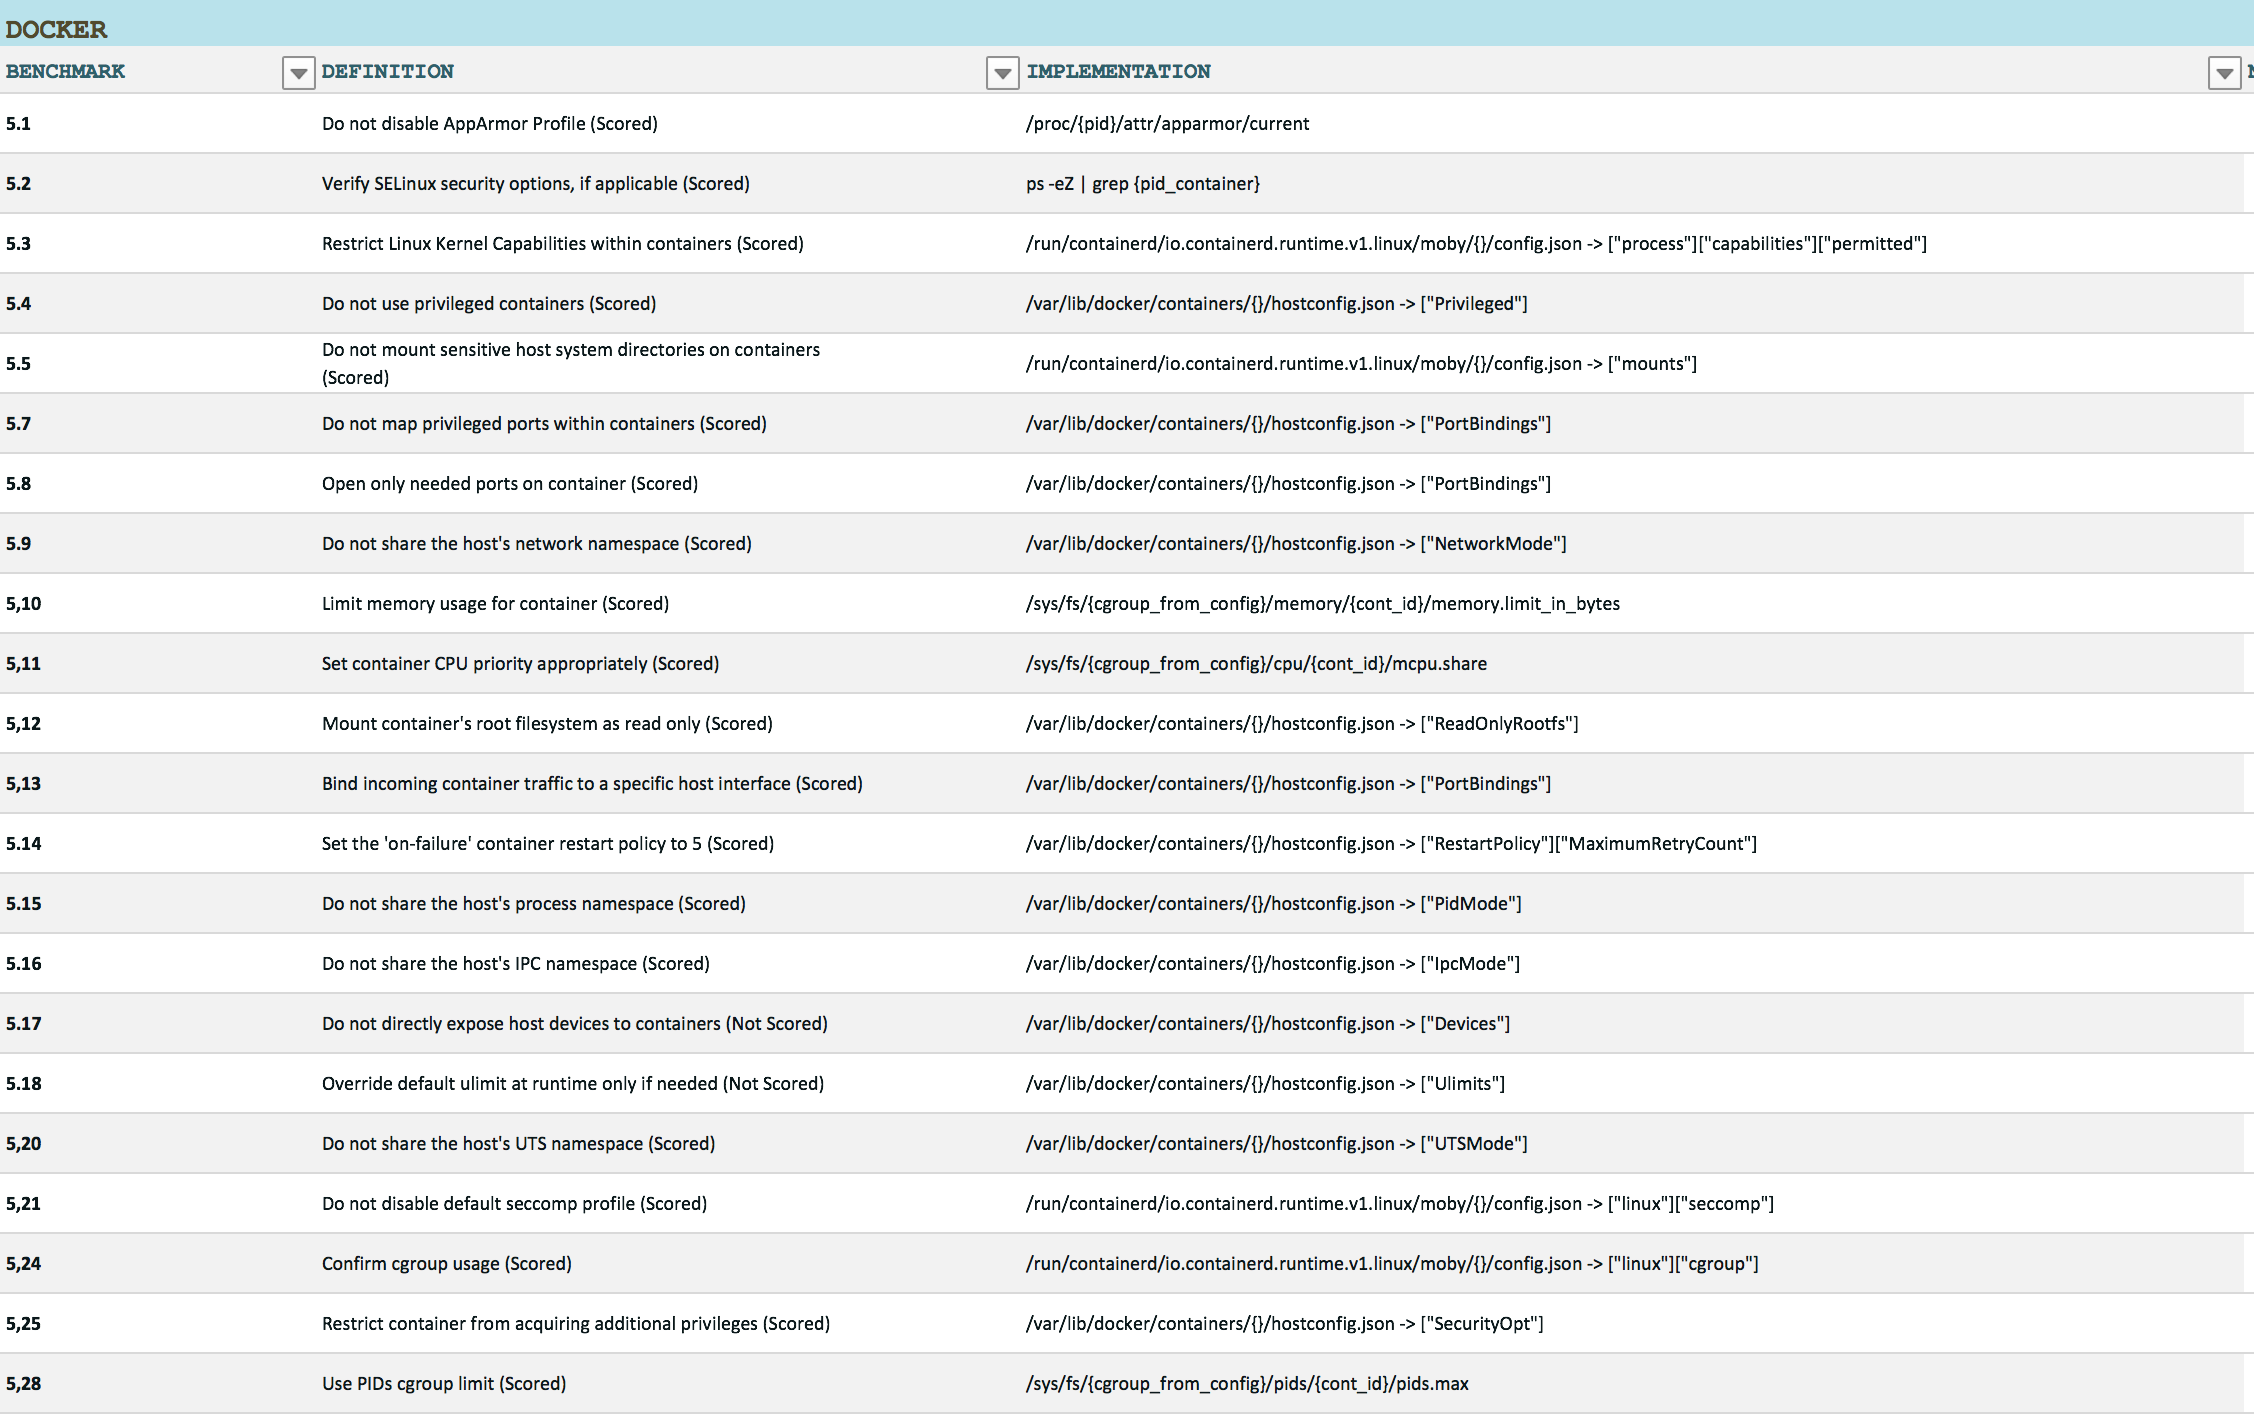
\includegraphics[width=\textwidth,height=10cm]{figures/docker}
  \end{figure*}


  \begin{figure*}
    \caption{CRIO.}
    \centering
      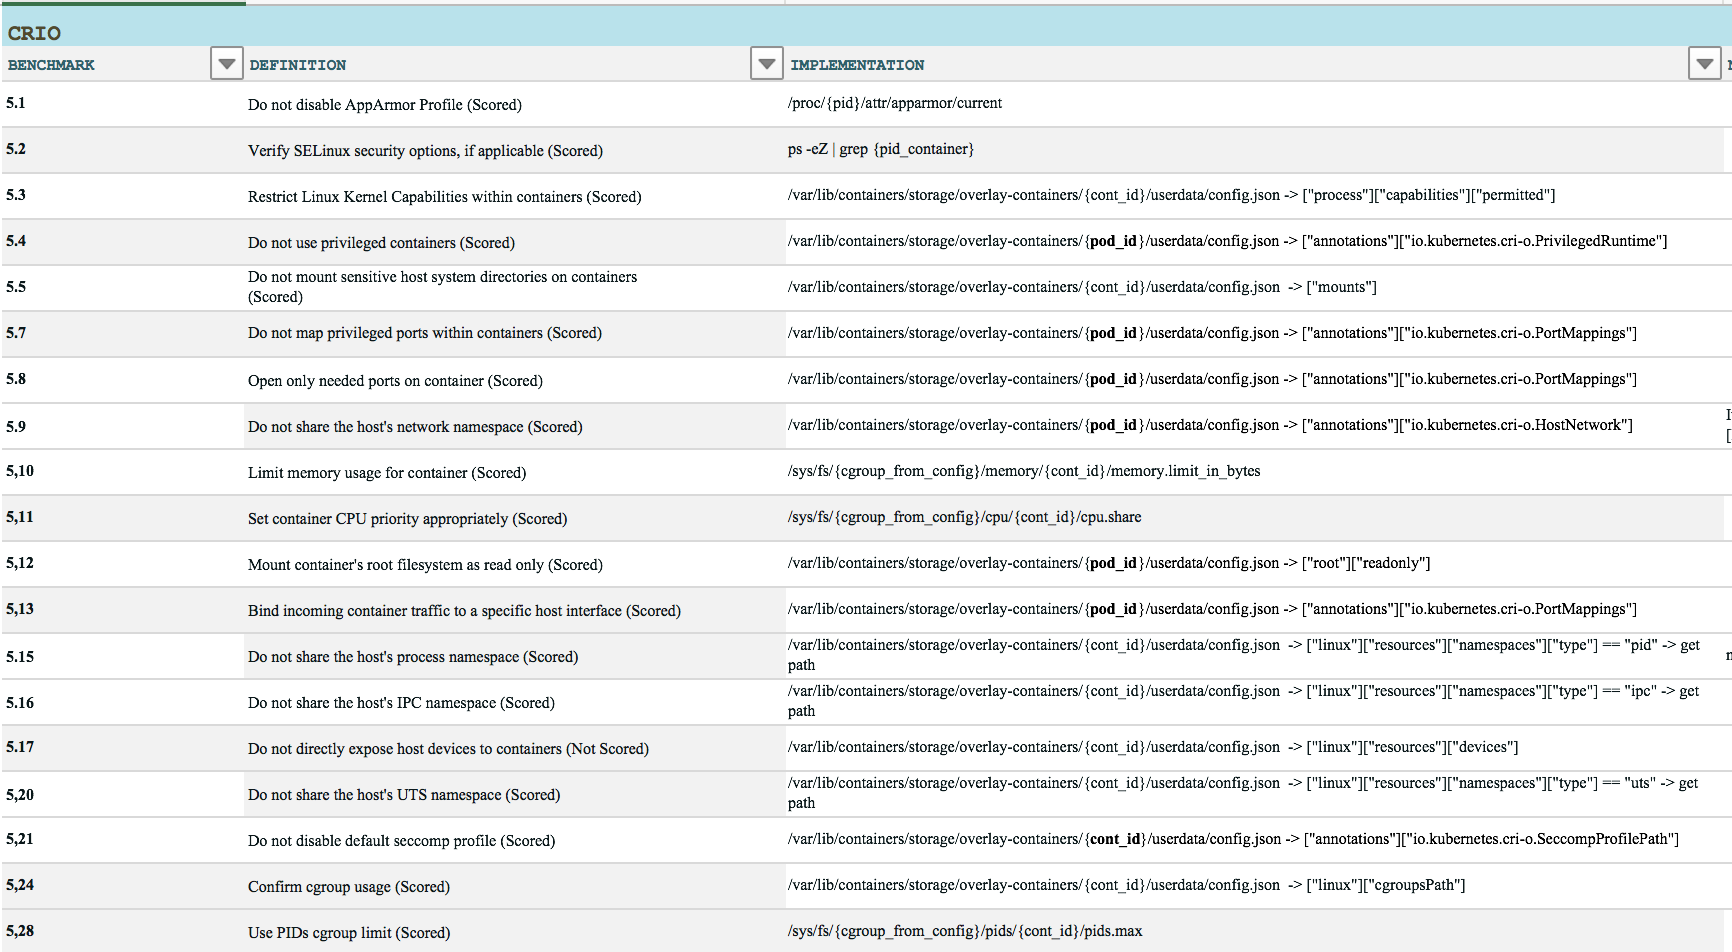
\includegraphics[width=\textwidth,height=10cm]{figures/crio}
  \end{figure*}


  \begin{figure*}
    \caption{Containerd}
    \centering
      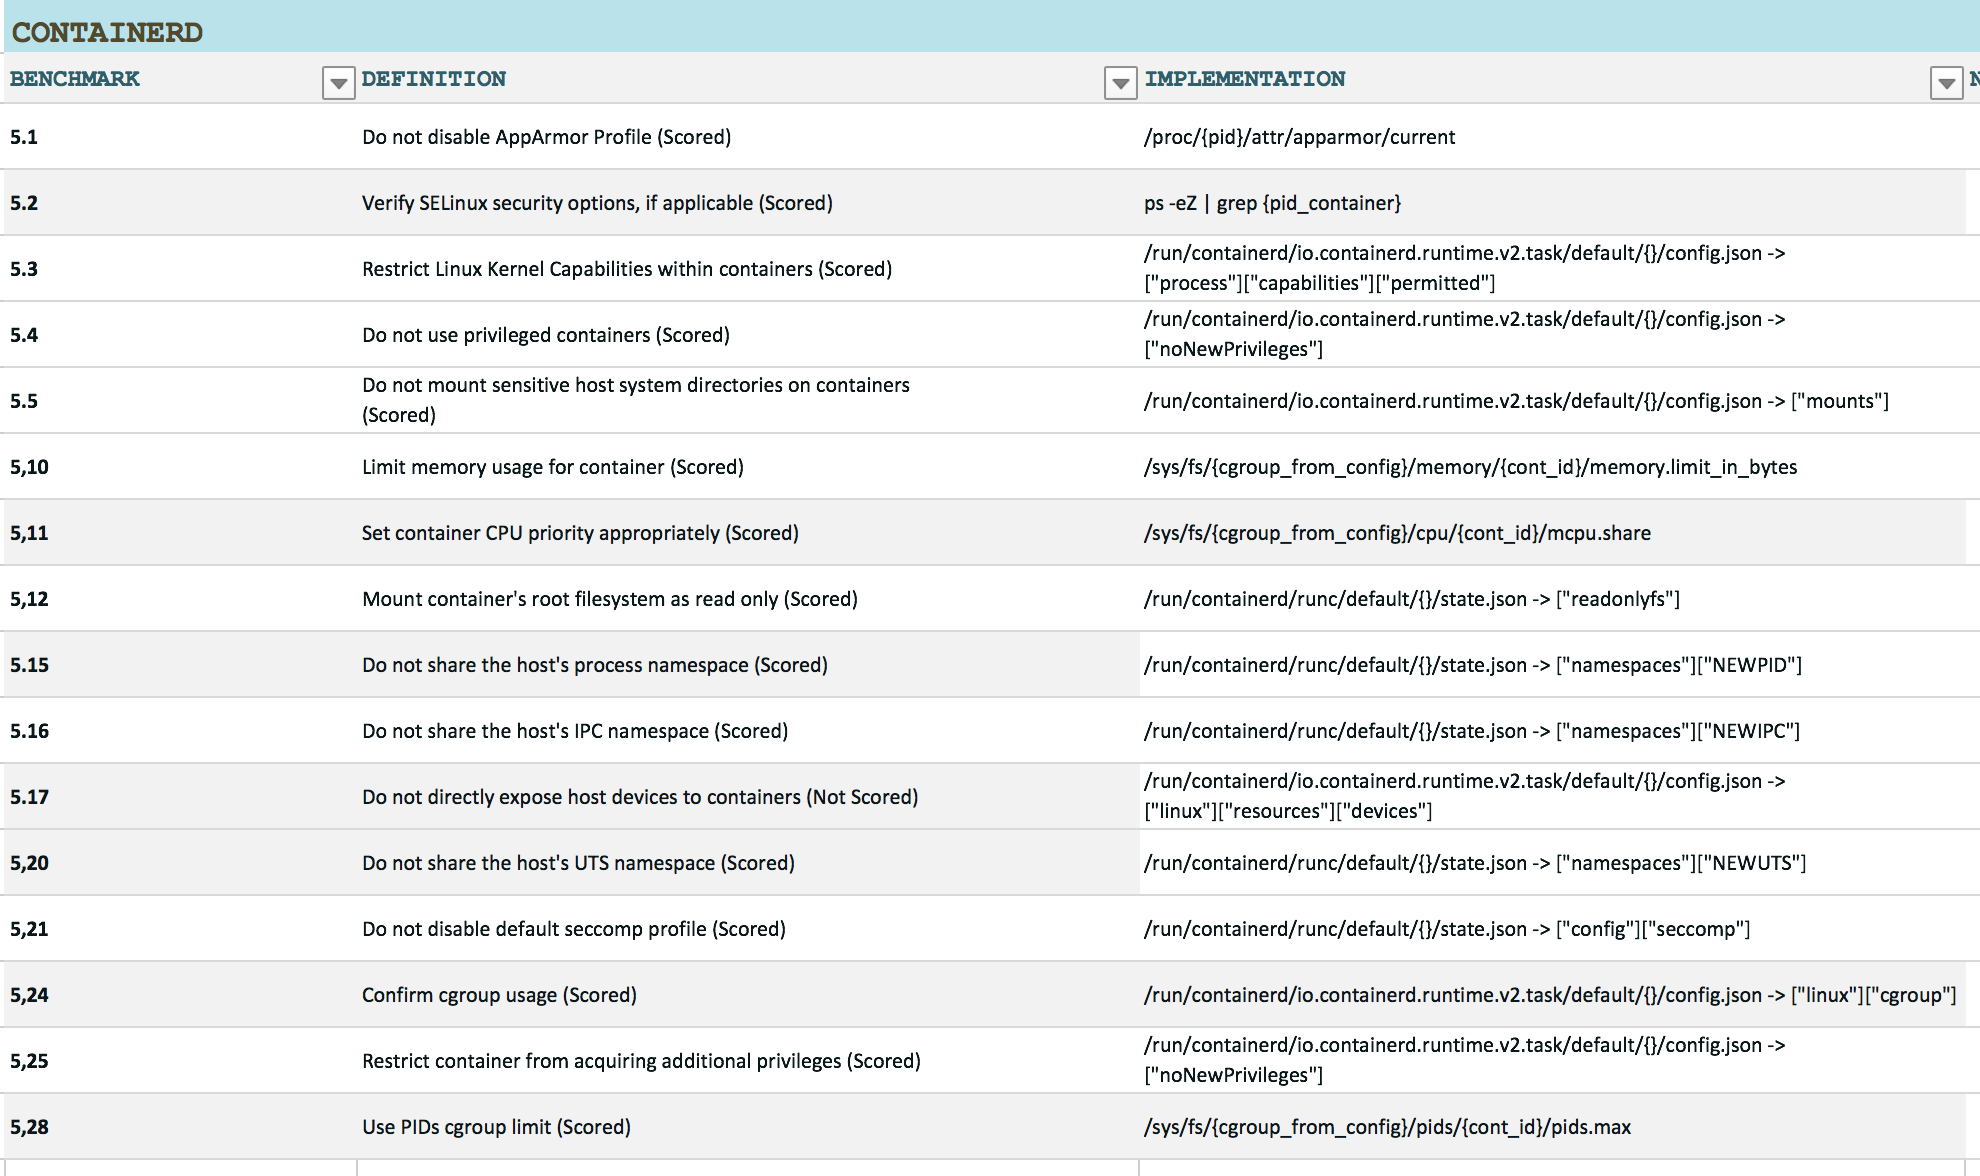
\includegraphics[width=\textwidth,height=10cm]{figures/containerd}
  \end{figure*}
\section*{Bibliography}

%% You can use these special %TC: tags to ignore certain parts of the text.
%TC:ignore
%the command above ignores this section for word count
\onecolumn
\newpage

%%%%%%%%%%%%%%%%%%%%%%%%%%%%%
% Supplementary Information %
%%%%%%%%%%%%%%%%%%%%%%%%%%%%%
\captionsetup*{format=largeformat}
\section{Something about something} \label{note:Note1} 
appendix

%TC:endignore
%the command above ignores this section for word count

\end{document}
